\section{Benchmark}

Performance evaluations is done with the benchmark program. For each tested data structure (presented in \cref{ch:numdb} and \cref{ch:alt}), the benchmark runs for a specified amount of time. Then the throughput (operations per second) is calculated as the total count of iterations divided by the total time.

Instead of separately measuring the performance of every basic operation (\findop, \insertop, \removeop), the overall numeric database performance is evaluated. The numeric database retrieval operation consists of either lookup (in case the item with the specified key is in the database) or lookup, user function invocation, item removal and item insertion. The user function is much slower than the database operations. Therefore, practically the most effective numerical database is the one that calls the user function as rarely as possible.

The recursive computation of the $N$th Fibonacci number is chosen as the user function. This algorithm implementation is trivial. Having the exponential time complexity it is extremely inefficient. This is the advantage from the perspective of the benchmark as its task is to simulate a very computational-heavy function. What is more, the time it takes to compute the function can be easily adjusted by the function argument.

Generally, cache systems perform well only on skewed inputs, when there is a small subset of items that are accessed most of the time while other items are accessed much less often. In this benchmark, a numerical database is tested with a random input sequence that has normal distribution of values. The parameters of the distribution are as follows:
\begin{description}
\item[Mean $u$] equals zero. The data structures presented in this library are agnostic to the particular argument values and their performance is only affected by the frequency of items in the input sequence. So $u$ can be any number. Zero is any number.

\item [Standard deviation $\sigma$] is derived from $Area{\mhyphen}under{\mhyphen}curve$ parameter and the available memory. $Capacity$ is calculated as the available memory divided by the size of a single item. $Area{\mhyphen}under{\mhyphen}curve$ is a value from the interval $(0,1)$. It defines the ratio of accesses to the $Capacity$ most valuable items to the total count of accesses. With given $Capacity$ and $Area{\mhyphen}under{\mhyphen}curve$, $\sigma$ is calculated as follows:
\begin{equation}
 \sigma = \frac{Capacity}{2 \times Quantile(0.5 + \frac{Area{\mhyphen}under{\mhyphen}curve}{2})}
 \end{equation}
\end{description}

\section{Benchmark Parameters}
The benchmark has several input parameters:
\begin{description}
\item [minval, maxval]-- the range of values the Fibonacci function is called with. It is defined as a range to simulate functions which execution time depends on its arguments.
\item [available memory]-- the maximum amount of memory the numerical database uses.
\item [thread count]-- relevant for concurrent numerical databases. Sets the number of  threads to run in parallel.
\item[mean changing rate]-- adjusts the rate at which the mean of the distribution is changed. If larger than zero, it simulates input sequences with non-static distribution. Measured as \emph{delta-per-iteration}~-- its value is added to the mean at every iteration, e.g. if the rate is $^1/_{100}$, than after 1000 iteration the mean will move by 10.
\item[area-under-curve]-- the parameter that affects the standard deviation of the distribution.
\end{description}

\pagebreak

The performance evaluation is performed on these machines:
\begin{itemize}
\item Single-threaded benchmarks
    \begin{description}
    \item [CPU] Intel\textsuperscript{\textregistered{}} Core\textsuperscript{\texttrademark{}} i5-6200U \\
    2.30GHz (2.80 GHz\footnote{with Intel\textsuperscript{\textregistered{}} Turbo Boost})$ \times$ 2 cores
    \item [Memory] 8 GB DDR3 1600 MHz
    \item [OS] Linux\textsuperscript{\textregistered{}} Ubuntu\textsuperscript{\textregistered{}} 16.04 LTS 64-bit
    \end{description}
\item Multi-threaded benchmarks
    \begin{description}
    \item [CPU] Intel\textsuperscript{\textregistered{}} Xeon\textsuperscript{\textregistered{}} E5-2650 v4 \\
    2.20GHz (2.90 GHz\footnotemark[1]) $ \times $ 2 sockets $ \times $ 12 cores
    \item [Memory] 256 GB DDR4 2400 MHz
    \item [OS] Linux\textsuperscript{\textregistered{}} Ubuntu\textsuperscript{\textregistered{}} 16.04 LTS 64-bit
    \end{description}
\end{itemize}

\section{Analysis}
\label{sec:banalysis}

Complete benchmark results are presented in appendix A. In this section they are analyzed.

\begin{center}
    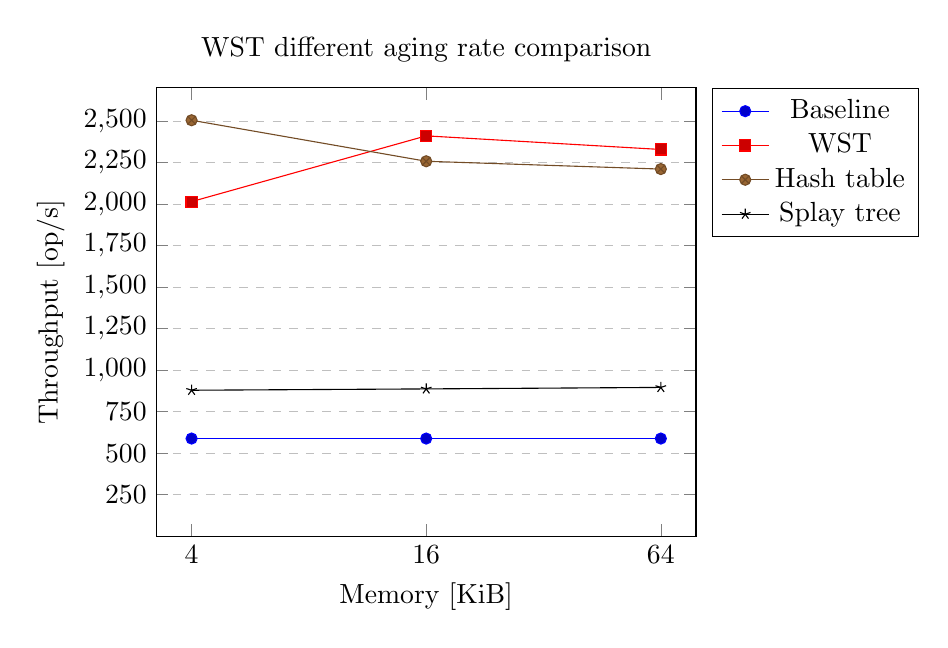
\begin{tikzpicture}
      \begin{axis}[
        legend pos=outer north east,
        title={\libname{WST} different aging rate comparison},
        xlabel = Memory {[KiB]},
        ylabel = Throughput {[op/s]},
        xmin = 0.85, xmax = 3.15,
        xtick={1,2,3},
        xticklabels={4, 16, 64},
        ymin = 0, ymax = 2700,
        ytick={250, 500, 750, 1000, 1250, 1500, 1750, 2000, 2250, 2500},
        ymajorgrids=true,
        grid style=dashed,
      ]
        \addplot coordinates{(1, 588)(2, 588)(3, 588)};
        \addplot coordinates{(1, 2015)(2, 2411)(3, 2329)};
        \addplot coordinates{(1, 2505)(2, 2258)(3, 2211)};
        \addplot coordinates{(1, 879)(2, 887)(3, 896)};
        \legend{Baseline,WST,Hash table,Splay tree}
      \end{axis}
      \end{tikzpicture}

    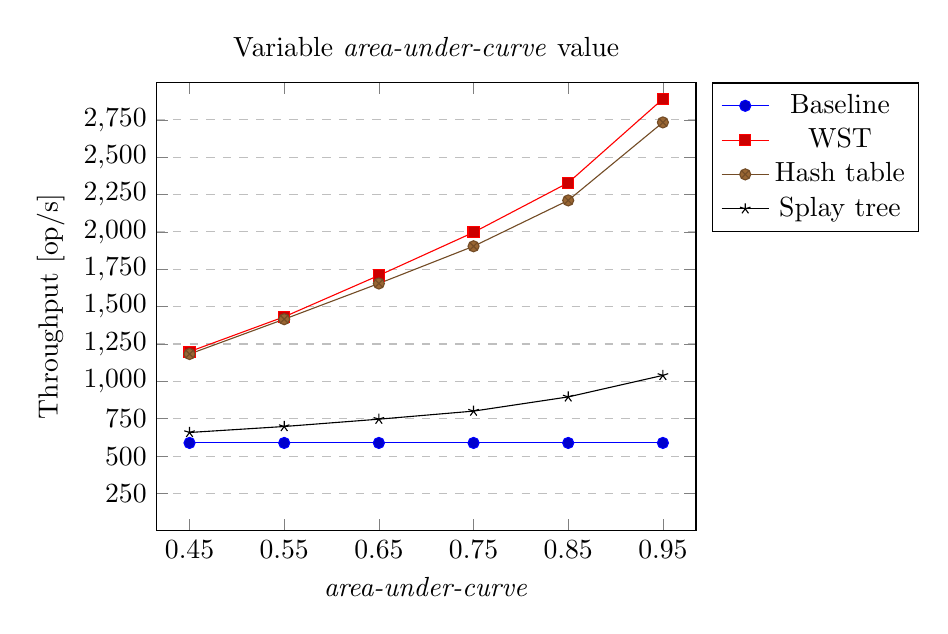
\begin{tikzpicture}
      \begin{axis}[
        legend pos=outer north east,
        title={Variable \emph{area-under-curve} value},
        xlabel = \emph{area-under-curve},
        ylabel = Throughput {[op/s]},
        xmin = 0.65, xmax = 6.35,
        xtick={1,2,3,4,5,6},
        xticklabels={0.45, 0.55, 0.65, 0.75, 0.85, 0.95},
        ymin = 0, ymax = 3000,
        ytick={250, 500, 750, 1000, 1250, 1500, 1750, 2000, 2250, 2500, 2750},
        ymajorgrids=true,
        grid style=dashed,
      ]
        \addplot coordinates{(1, 588)(2, 588)(3, 588)(4, 588)(5,588)(6,588)};
        \addplot coordinates{(1, 1199)(2, 1432)(3, 1709)(4, 1997)(5,2329)(6,2890)};
        \addplot coordinates{(1, 1183)(2, 1416)(3, 1655)(4, 1904)(5,2211)(6,2733)};
        \addplot coordinates{(1, 658)(2, 698)(3, 747)(4, 801)(5,896)(6,1040)};
        \legend{Baseline,WST,Hash table,Splay tree}
      \end{axis}
    \end{tikzpicture}

    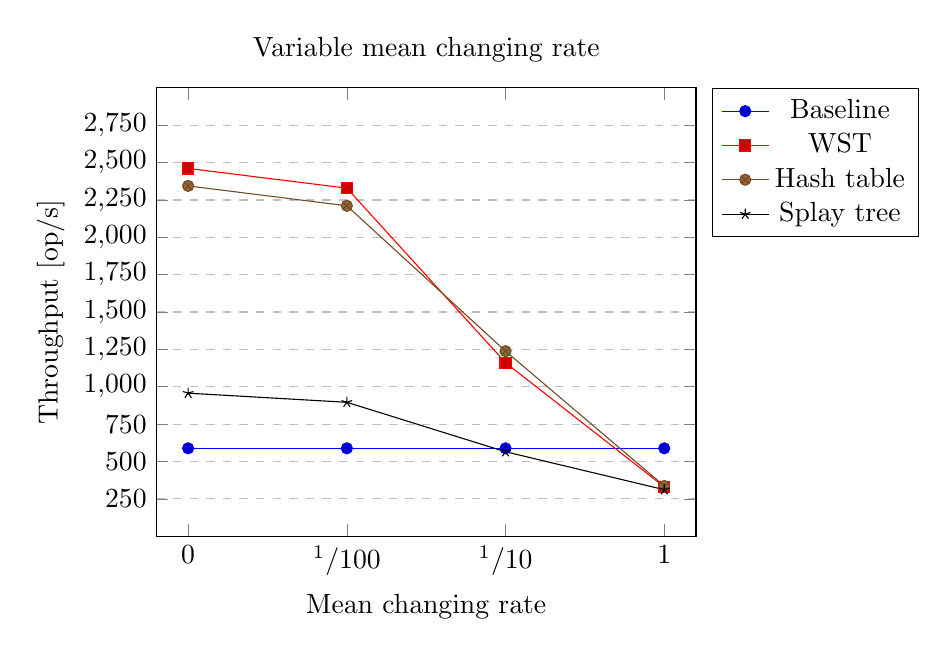
\begin{tikzpicture}
          \begin{axis}[
            legend pos=outer north east,
            title={Variable mean changing rate},
            xlabel = Mean changing rate,
            ylabel = Throughput {[op/s]},
            xmin = 0.80, xmax = 4.20,
            xtick={1,2,3,4},
            xticklabels={0, $^1/{100}$, $^1/{10}$, 1},
            ymin = 0, ymax = 3000,
            ytick={250, 500, 750, 1000, 1250, 1500, 1750, 2000, 2250, 2500, 2750},
            ymajorgrids=true,
            grid style=dashed,
          ]
            \addplot coordinates{(1, 588)(2, 588)(3, 588)(4, 588)};
            \addplot coordinates{(1, 2461)(2, 2329)(3, 1161)(4, 330)};
            \addplot coordinates{(1, 2344)(2, 2211)(3, 1238)(4, 336)};
            \addplot coordinates{(1, 957)(2, 896)(3, 565)(4, 311)};
            \legend{Baseline,WST,Hash table,Splay tree}
          \end{axis}
        \end{tikzpicture}
\end{center}

\begin{description}
\item[Splay tree]The experimental evaluation proved splay tree ineffeciency. It is outperformed by WST and the hash table on all workloads. Therefore it is not recommended to use it for a numerical database.
\item[Alternative eviction strategies] LRU and LFU strategies turned out to be impractical from the perspective of numerical databases. The possible reason is that these policies discard initial priority and rely solely on access frequency.
\item[WST] This data structure proved to be the most effective for a numerical database. However, no concurrent WST implementation is known, so it may be used in sequantial systems only.
\item[Hash table] In combination with a binary heap this data structure achieves approximately same throughput (about 10\% lower) as WST. The concurrent version of this container has been introduced in this thesis.
\item[Mean changing rate] With the rate greater or equal 1, the numerical database becomes impractical~-- it achieves only half of the baseline performance.
\item[Priority aging] Priority aging does not show any advantage over static priority. However, further studies and tests are required here, as the benchmark did not simulate the worst-case input for the static priority scheme.
\end{description}
